\section{Design of timber bridges}\label{sec:ponte_madeira}

This section presents the design criteria adopted for roundwood log-girder timber bridges, covering the design vehicle actions, the partial factors for the mechanical properties, the deflection limits and the verification procedure of the girder and the deck.

\subsection{Design vehicle load}\label{sec:trem_tipo}

The moving loads of Brazilian highway bridges are defined by \textcite{nbr7188} in its item 5.1.1. Since the bridges considered serve low-traffic rural roads, the TB-240 design vehicle is adopted. It is characterized by a 240~kN vehicle with six wheels and three axles, a load of 40~kN per wheel and an axle spacing of 1.5~m, complemented by a uniformly distributed crowd load of 4.0~kN/m\textsuperscript{2} around it, as shown in Fig.~\ref{fig:trem}.

\begin{figure}[htpb!]
\centering
\begin{subfigure}{0.30\textwidth}
    \centering
    
\includegraphics[width=\textwidth]{figuras/trem_elevacao.png}
    \caption{Elevation.}
    \label{fig:trem_elevacao}
\end{subfigure}
\hspace{0.02\textwidth}
\begin{subfigure}{0.30\textwidth}
    \centering
    
\includegraphics[width=\textwidth]{figuras/trem_planta.png}
    \caption{Plan (6.00~$\times$~3.00~m = 18.0~m\textsuperscript{2}).}
    \label{fig:trem_planta}
\end{subfigure}
\caption{Configuration of the TB-240 design vehicle \parencite{nbr7188}.}
\label{fig:trem}
\end{figure}

\subsection{Partial factors for mechanical properties}

For the structural checks, \textcite{NBR7190-1:2022} establishes strength ($f$) and modulus of elasticity ($E$) parameters for softwoods and hardwoods under the standard reference condition, that is, a moisture content ($U$) of 12\%.
The limit state method amplifies the internal forces and reduces these strengths by the modification factor ($k_{\mathrm{mod}}$) and the material partial factor ($\gamma_w$), according to Eq.~\eqref{eq:2.099}, where $X_k$ is the characteristic strength and $\gamma_w$ equals 1.4 for normal stresses and 1.8 for shear stresses.

\begin{equation}
    X_d = \frac{k_{\mathrm{mod}} \cdot X_k}{\gamma_w}
\label{eq:2.099}
\end{equation}

The modification factor is the product $k_{\mathrm{mod},1}\cdot k_{\mathrm{mod},2}$ (Eq.~\eqref{eq:2.99}), where the first factor depends on the load-duration class (item 5.8.4.1 of \textcite{NBR7190-1:2022}) and the second on the moisture class (item 5.8.4.2).

\begin{equation}
k_{\mathrm{mod}} = k_{\mathrm{mod},1} \cdot k_{\mathrm{mod},2}
\label{eq:2.99}
\end{equation}

\textcite{NBR7190-1:2022} does not explicitly classify road traffic actions with respect to their cumulative duration. The classification of item 2.3.1.2 of \textcite{EN1995-2:2004} and item NA.2.1 of the UK National Annex \textcite{BSNA-EN1995-2:2004} is adopted here, which treat actions from vehicles and pedestrians as \emph{short-term actions} owing to their transient and non-sustained nature, yielding $k_{\mathrm{mod},1} = 0.90$ for solid timber.
For the adopted moisture class (3), compatible with structural members exposed to the weather but protected from direct contact with water, a condition typical of roundwood bridges on rural roads, $k_{\mathrm{mod},2} = 0.80$.

\subsection{Deflection limits}\label{sec:flecha_limite}

\subsubsection{Creep}

The instantaneous deflections, $\delta_{\mathrm{inst},G_i,k}$ and $\delta_{\mathrm{inst},Q_j,k}$, associated with permanent and variable actions respectively, are computed with the mean modulus of elasticity in bending, $E_{0,\mathrm{m}}$. The effect of time on stiffness is incorporated separately through the creep coefficient $\varphi$, which amplifies the instantaneous deflections to obtain the final deflections $\delta_{\mathrm{fin},G_i,k}$ and $\delta_{\mathrm{fin},Q_j,k}$, according to Eqs.~\eqref{eq:flecha_fin_G} and~\eqref{eq:flecha_fin_Q}.

\begin{equation}
\delta_{\mathrm{fin},G_i,k}
=
\delta_{\mathrm{inst},G_i,k}
+ \delta_{\mathrm{creep}}
=
\delta_{\mathrm{inst},G_i,k} \cdot (1 + \varphi)
\label{eq:flecha_fin_G}
\end{equation}

\begin{equation}
\delta_{\mathrm{fin},Q_j,k}
=
\delta_{\mathrm{inst},Q_j,k}
+ \delta_{\mathrm{creep}}
=
\delta_{\mathrm{inst},Q_j,k} \cdot \psi_{2} \cdot (1 + \varphi)
\label{eq:flecha_fin_Q}
\end{equation}

According to \textcite{NBR7190-1:2022}, timber has characteristics distinct from other construction materials, such as significant time-dependent deformation (creep).
The creep coefficient $\varphi$ (item 8.1, Table 20 of \textcite{NBR7190-1:2022}) is defined as a function of the material and of the moisture class of the structure, increasing for higher moisture classes. For the moisture class (3) adopted in this work and for sawn timber or roundwood, the reference value is $\varphi = 0.8$.

\subsubsection{Code deflection limits}

For the serviceability limit state (SLS) check, item 8.2 of \textcite{NBR7190-1:2022} establishes limit values for the instantaneous deflection ($\delta_{\mathrm{inst}}$) and the final deflection ($\delta_{\mathrm{fin}}$), which depend on the static configuration of the structure.
For simply supported or continuous beams, which is the case of the structural system analysed in this work, the code interval lies between $L/300$ and $L/500$ for $\delta_{\mathrm{inst}}$ and between $L/150$ and $L/300$ for $\delta_{\mathrm{fin}}$. The specific values adopted in this work are presented in Section~\ref{sec:projeto_ponte} (Eq.~\eqref{eq:verflecha}).

\subsection{Bridge design}\label{sec:projeto_ponte}

The structural system considered consists of a deck of rectangular timber planks, of width $b_w$ and height $h$, continuously supported on circular roundwood girders of diameter $d$, analysed as simply supported beams of span $L$.
The verification steps follow the sequence of determination of the internal forces, bending and shear checks of the girder, deflection check and, finally, bending check of the deck.
The calculation procedure presented in this section follows the code criteria of \textcite{NBR7190-1:2022} and the design procedure of the timber bridge design and construction manual by \textcite{CALIL2006}.

\subsubsection{Internal forces}

For the solid circular girder and the rectangular deck plank, the area, second moment of area and section modulus of the cross-sections follow the usual geometric expressions for circular and rectangular sections, respectively.

The permanent actions correspond to the self-weight of the girders, the deck and other members, obtained from the geometry and the unit weight $\gamma$, according to Eq.~\eqref{eq:permanente}.

\begin{equation}
G = \gamma \cdot A
\label{eq:permanente}
\end{equation}

The moving load considered is the TB-240 design vehicle presented in Section~\ref{sec:trem_tipo}, represented by a three-axle, six-wheel vehicle, each wheel transmitting a load $P$ of 40~kN, together with the crowd load, uniformly distributed over the occupation area with the characteristic value $q_A = 4.0$~kN/m\textsuperscript{2}.
Since the girders are treated as isolated beams, the crowd load must be converted from an area load into a line load before entering Eqs.~\eqref{eq:mqk45} and~\eqref{eq:qqkenv}, by multiplying $q_A$ by the tributary width of each girder, that is, by the corrected girder spacing $esp_{long,corr}$ (Section~\ref{sec:formulacao}), according to Eq.~\eqref{eq:qlong}.

\begin{equation}
q = q_A \cdot esp_{long,corr}
\label{eq:qlong}
\end{equation}

Dynamic effects are incorporated through the vertical impact coefficient ($CIV$), determined by Eqs.~\eqref{eq:civ1} and~\eqref{eq:civ2} according to item 5.1.3.1 of \textcite{nbr7188}, where $LIV$ is the characteristic length of the structure.

\begin{equation}
CIV = 1.35 \qquad \text{for } L \leq 10.0\ \text{m}
\label{eq:civ1}
\end{equation}

\begin{equation}
CIV = 1 + 1.06\left(\frac{20}{LIV + 50}\right), \qquad \text{for } 10.0 < L \leq 200.0\ \text{m}
\label{eq:civ2}
\end{equation}

The $CIV$ directly multiplies the internal forces due to variable actions.

The maximum bending moment and shear force due to the permanent load, as well as the corresponding static deflection, are obtained from classical statics of simply supported beams, according to Eqs.~\eqref{eq:mgk} and~\eqref{eq:qgk}.

\begin{equation}
M_{gk} = \frac{g\,L^2}{8}
\label{eq:mgk}
\end{equation}

\begin{equation}
Q_{gk} = \frac{g\,L}{2}
\label{eq:qgk}
\end{equation}

The effects of the design vehicle are determined using structural analysis concepts and the recommendations of \textcite{CALIL2006}.

\subsubsection*{Bending moment and deflection}

For the bending moment and the deflection, the vehicle is centred on the span, with the central wheel located exactly at midspan and the two outer wheels at a distance $a$ from it, as shown in Fig.~\ref{fig:posicao_momento_flecha}.

\begin{figure}[!ht]
    \centering
    \begin{subfigure}{0.46\textwidth}
        \centering
        
\includegraphics[width=\textwidth]{figuras/posicionamento_momento_flecha.png}
        \caption{Bending moment and deflection.}
        \label{fig:posicao_momento_flecha}
    \end{subfigure}
    \hfill
    \begin{subfigure}{0.46\textwidth}
        \centering
        
\includegraphics[width=\textwidth]{figuras/posicionamento_cortante.png}
        \caption{Shear force.}
        \label{fig:posicao_cortante}
    \end{subfigure}
    \caption{Positioning of the design vehicle for computing the girder internal forces \parencite{CALIL2006}.}
    \label{fig:posicionamentos}
\end{figure}

The maximum bending moment under the central wheel results from Eq.~\eqref{eq:mqk30}, written for $3\,\text{m} < L \leq 6\,\text{m}$. For spans greater than 6~m, Eq.~\eqref{eq:mqk45} gives the maximum moment.

\begin{equation}
c = \frac{L - 4a}{2}, \qquad \text{for } L > 6\,\text{m}
\label{eq:cmomento}
\end{equation}

\begin{equation}
M_{qk} = \frac{3\,P\,L}{4} - P\,a, \qquad \text{for } 3\,\text{m} < L \leq 6\,\text{m}
\label{eq:mqk30}
\end{equation}

\begin{equation}
M_{qk} = \left(\frac{3\,P\,L}{4} - P\,a\right) + \frac{q\,c^2}{2}, \qquad \text{for } L > 6\,\text{m}
\label{eq:mqk45}
\end{equation}

The centred position, however, is the position of maximum moment only while the three wheels actually load the span. With the outer wheels at $L/2 \pm a$ from the left support, they reach the supports when $L = 2a$. From then on they have zero lever arm, or leave the span, and the centred arrangement no longer maximizes the moment. For $a = 1.5$~m and $L = 3.0$~m, the outer wheels rest exactly on the supports and Eq.~\eqref{eq:mqk30} degenerates into the case of a single centred load, $M_{qk} = PL/4$.

In this case, the maximum moment is found by positioning the design vehicle so that only two wheels lie within the span, following Barré's theorem, according to which the midspan must lie exactly halfway between one of the loads and the resultant of the pair. This condition leads to the position $x = (2L-a)/4$ for the first wheel, and the maximum moment is given by Eq.~\eqref{eq:mqk2}, obtained by maximizing $M(x) = P\,x\,(2L - 2x - a)/L$.

\begin{equation}
M_{qk}^{(2)} = \frac{P\,(2L-a)^2}{8L}, \qquad \text{valid for } L \geq 1.5\,a
\label{eq:mqk2}
\end{equation}

The envelope of the moment due to the moving load is therefore the largest value among the admissible arrangements, namely three centred wheels, two wheels in Barré's position, or a single wheel at midspan, according to Eq.~\eqref{eq:mqkenv}.

\begin{equation}
M_{qk} = \max\left(\frac{3PL}{4} - Pa\;,\;\; \frac{P\,(2L-a)^2}{8L}\;,\;\; \frac{PL}{4}\right)
\label{eq:mqkenv}
\end{equation}

The first term governs for $L \geq 2.23\,a$, that is, $L \geq 3.34$~m when $a = 1.5$~m, so that Eq.~\eqref{eq:mqkenv} recovers Eq.~\eqref{eq:mqk30} over the usual range and differs from it only for the shortest spans. For the 3.0~m span, the centred formulation gives $30.0$~kN$\cdot$m against $33.75$~kN$\cdot$m from the envelope, an underestimation of $12.5\%$. For $L > 6$~m, where the crowd load contribution appears, the centred arrangement governs by a wide margin and Eq.~\eqref{eq:mqk45} remains governing.

The same centred position of Fig.~\ref{fig:posicao_momento_flecha} is used for the deflection (Section~\ref{sec:formulacao}, Eqs.~\eqref{eq:flechag} and~\eqref{eq:flechaq}), with $b$ the distance between the support and the nearest outer wheel.

\subsubsection*{Shear force}

For the shear force, Fig.~\ref{fig:posicao_cortante} shows the vehicle placed at a distance $2h$ from the support, where $h$ is the depth (or the diameter, for a circular section) of the member, the position at which \textcite{NBR7190-1:2022} allows the shear force to be evaluated instead of at the face of the support itself.
Since the diameter of the roundwood girder is not negligible compared with the span in the range of interest of this work, the design shear force $Q_{qk}$ is obtained directly from Eq.~\eqref{eq:qqkenv}, in which the operator $\max(\cdot\,,0)$ cancels the contribution of the wheels and of the crowd load segment that exceed the finite length of the span.

\begin{equation}
\begin{split}
Q_{qk} = \frac{P}{L}\Big[\max(L-2h,\,0) + \max(L-2h-a,\,0) &+ \max(L-2h-2a,\,0)\Big] \\
&+ \frac{q}{2L}\Big[\max(L-2h-3a,\,0)\Big]^{2}
\end{split}
\label{eq:qqkenv}
\end{equation}

The design internal forces, $M_{sd}$ and $Q_{sd}$, follow the code load combination of \textcite{NBR8681:2025}.
For a single-span bridge subjected to self-weight and to the design vehicle as the only leading variable action, this combination reduces to Eq.~\eqref{eq:comb}, where $\gamma_g = 1.30$ and $\gamma_q = 1.50$ are the partial factors for permanent and variable actions, respectively.

\begin{equation}
M_{sd} = \gamma_g\,M_{gk} + \gamma_q\,M_{qk}, \qquad Q_{sd} = \gamma_g\,Q_{gk} + \gamma_q\,Q_{qk}
\label{eq:comb}
\end{equation}

\subsubsection{Bending design}

The design bending strength, $f_{md}$, is obtained from the characteristic strength $f_{mk}$ multiplied by the modification factor $k_{\mathrm{mod}}$ and divided by the partial factor $\gamma_w$, as already presented in Eq.~\eqref{eq:2.099}.
The bending check of the girder compares the design normal stress with this strength, according to Eq.~\eqref{eq:verflexao}.

\begin{equation}
\frac{\sigma_{Mx,d}}{f_{md}} = \frac{M_{sd}}{W_x\,f_{md}} \leq 1
\label{eq:verflexao}
\end{equation}

\subsubsection{Shear design}

For the solid circular section, the maximum shear stress occurs at the neutral axis and is compared with the design shear strength, $f_{v0,d}$, according to Eq.~\eqref{eq:vercis}.

\begin{equation}
\tau_{\max} = \frac{4}{3}\,\frac{Q_{sd}}{A} \leq f_{v0,d}
\label{eq:vercis}
\end{equation}

\subsubsection{Deflection design}

The deflections due to the permanent load ($\delta_{gk}$) and to the concentrated moving load ($\delta_{qk}$) on the girder are obtained from Eqs.~\eqref{eq:flechag} and~\eqref{eq:flechaq}, where $E_{0,\mathrm{m}}$ is the mean modulus of elasticity in bending and $b$ is the distance between the support and the load application point, defined by Eq.~\eqref{eq:bflecha}.

\begin{equation}
\delta_{gk} = \frac{5\,g\,L^4}{384\,E_{0,\mathrm{m}}\,I}
\label{eq:flechag}
\end{equation}

\begin{equation}
b = \frac{L - 2a}{2}
\label{eq:bflecha}
\end{equation}

\begin{equation}
\delta_{qk} = \frac{P}{48\,E_{0,\mathrm{m}}\,I}\left[L^3 + 2\,b\left(3L^2 - 4b^2\right)\right]
\label{eq:flechaq}
\end{equation}

These contributions correspond to the instantaneous deflections used in Eqs.~\eqref{eq:flecha_fin_G} and~\eqref{eq:flecha_fin_Q}, whose sum gives the total deflection $\delta_{\mathrm{fin}}$ already including creep.
The deflection check simultaneously compares this total deflection, in the quasi-permanent combination, with the code limit $L/350$, and the total instantaneous deflection, $\delta_{\mathrm{inst}} = \delta_{gk} + \delta_{qk}$, due to permanent and variable actions in the characteristic (rare) combination without creep, with the limit $L/500$, both from Table 21 of \textcite{NBR7190-1:2022}, according to Eq.~\eqref{eq:verflecha}.

\begin{equation}
\max\left(\frac{\delta_{\mathrm{fin}}}{L/350},\ \frac{\delta_{gk} + \delta_{qk}}{L/500}\right) \leq 1
\label{eq:verflecha}
\end{equation}

\subsubsection{Deck design}

The deck plank is checked in isolation as a simply supported beam spanning the girder spacing ($esp_{long}$).
The bending moment due to the permanent load on the deck, $M_{gk,tab}$, follows the same formulation as Eq.~\eqref{eq:mgk}, replacing $L$ by $esp_{long}$.
The bending moment due to the concentrated load of one wheel of the design vehicle is obtained by placing a single wheel at the middle of this local span, as shown in Fig.~\ref{fig:posicao_tabuleiro}, the critical position for an isolated concentrated load on a simply supported beam.

\begin{figure}[!ht]
    \centering
    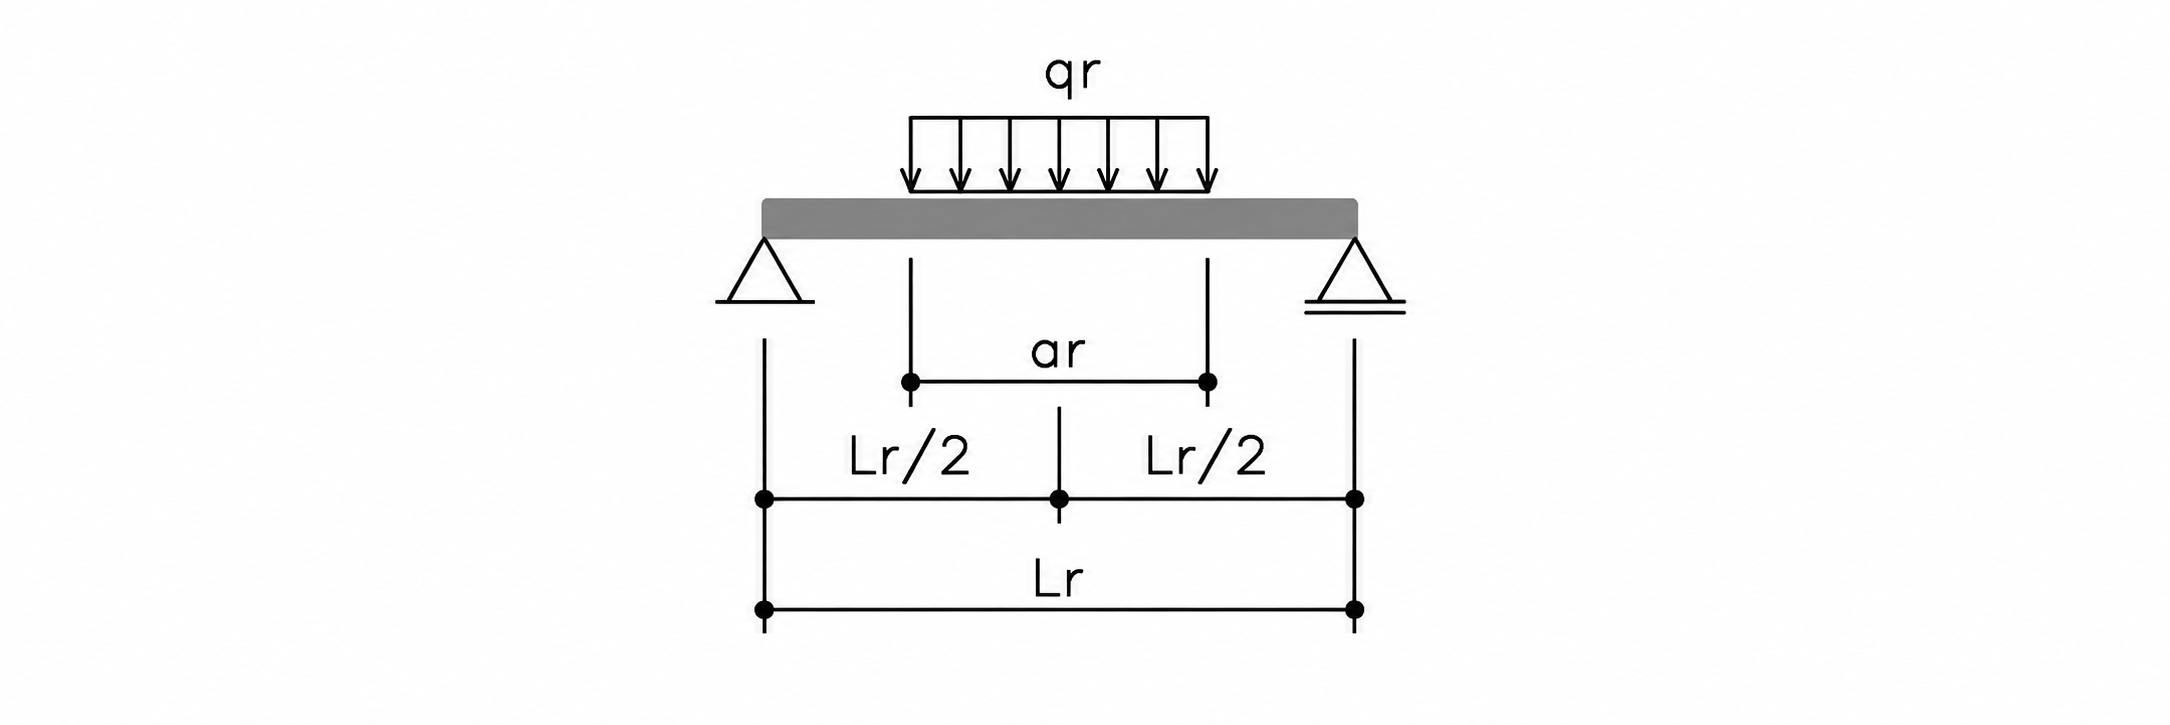
\includegraphics[trim=680bp 65bp 740bp 35bp,clip,width=0.15\textwidth]{figuras/posicionamento_roda_tabuleiro.png}
    \caption{Critical position of a wheel on the deck \parencite{CALIL2006}.}
    \label{fig:posicao_tabuleiro}
\end{figure}

$M_{qk,tab}$ is then obtained from Eq.~\eqref{eq:mqktab}, where $a_r$ is the effective contact length of the wheel on the deck and $CIV_{tab}$ is the vertical impact coefficient computed analogously to Eqs.~\eqref{eq:civ1} and~\eqref{eq:civ2}, taking the spacing $esp_{long}$ as the reference span.

\begin{equation}
M_{qk,tab} = \frac{P}{4}\,\left(esp_{long} - a_r\right)\cdot CIV_{tab}
\label{eq:mqktab}
\end{equation}

The design moment of the deck, $M_{sd,tab}$, follows the same load combination as Eq.~\eqref{eq:comb}.
The bending check of the deck follows the same criterion used for the girder (Eq.~\eqref{eq:verflexao}), comparing the design normal stress $\sigma_{x,d,tab} = M_{sd,tab}/W_{x,tab}$ with the design bending strength of the deck $f_{md,tab}$, computed according to Eq.~\eqref{eq:2.099}.
